Sometimes you end up looking at posts from the Fediverse best in blog
posts. Context really matters. Of course, the situation we find
ourselves in right now in the United States of America is a bad one.

Quoting
\href{https://kolektiva.social/@VPS_Reports/}{@VPS\_Reports@kolektiva.social}:
\url{https://kolektiva.social/@VPS_Reports/111814616001094165} \#retoot

\begin{figure}
\centering
\pandocbounded{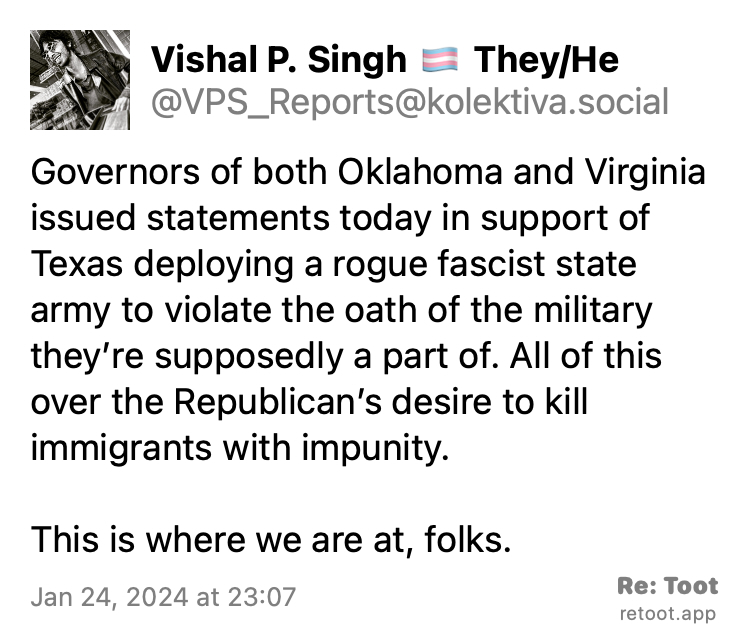
\includegraphics[keepaspectratio]{\%7B\%7Bsite.url\%7D\%7D/img/txguard.jpg}}
\caption{Post by Vishal P. Singh 🏳️‍⚧️ They/He. ``Governors of both
Oklahoma and Virginia issued statements today in support of Texas
deploying a rogue fascist state army to violate the oath of the military
they're supposedly a part of. All of this over the Republican's desire
to kill immigrants with impunity. This is where we are at, folks.''
Posted on Jan 24, 2024 at 23:07}
\end{figure}

\begin{quote}
\emph{Post by Vishal P. Singh 🏳️‍⚧️ They/He. ``Governors of both Oklahoma
and Virginia issued statements today in support of Texas deploying a
rogue fascist state army to violate the oath of the military they're
supposedly a part of. All of this over the Republican's desire to kill
immigrants with impunity. This is where we are at, folks.'' Posted on
Jan 24, 2024 at 23:07}
\end{quote}

This grossly over-simplifies and spins what is a hideously complicated
situation in Texas right now. First and foremost, you must remember that
the United States of America does \textbf{not} have one single military.
Each of the fifty states has its own militia forces. Most people think
that means \emph{solely} the dual-hatted National Guard which has both
state and federal roles. That's not entirely true as section 109 of
title 32 of the United States Code
\href{https://web.archive.org/web/20230519053302/https://www.law.cornell.edu/uscode/text/32/109}{authorizes
the maintenance and operation of ``state defense force'' formations}.
Not every state has chosen to operate its own state defense force but
Texas has
\href{https://web.archive.org/web/20231107171339/https://tmd.texas.gov/state-guard}{the
Texas State Guard}.

As far as can be seen, it is the Texas State Guard that is being
utilized to project the power of the state of Texas in the conflict with
the federal government over the southern border. The state government in
Texas is apparently trying to ensure they don't lose control of their
henchmen in the matter as using National Guard troops runs the risk of
federalization under various constitutional authorities and redeployment
by the Pentagon. Clashes like this easily bring up echoes of Fort Sumter
as well as the desegregation clash in 1957 in Arkansas.

What could possibly go wrong?
